There are two main sets of hyper-parameters to be tuned:
\begin{itemize}
    \item The number of features to use to fit each model is indicated by $n_{RI}$ and $n_{MLP}$.
    \item Ridge regressor and MLP regressor parameters
\end{itemize}
For tuning the parameters we considered a split of the development set into \textit{train} and \textit{validation} set, containing the 80\% and the 20\% of the points.

For convenience we assume that two set are independent, therefore we can first optimize the number of features used to fit the regressor and then perform some tuning of the hyper-parameters of the two regressor.

\begin{itemize}
    \item \textit{Ridge parameters}: Before finding the best parameters using a grid search, we found the best features for fitting the regression. We used a \textit{scikit-learn} class called \textit{RFE}\cite{RFE} (\textit{recursive features elimination}), to execute this task. We trained and tested the ridge model increasing the feasible number of features each time, obtaining that the best number of features is 50, as shown in Figure \ref{num vs rmse}. The feature selection has been performed by using the default parameters.
    \begin{figure}
    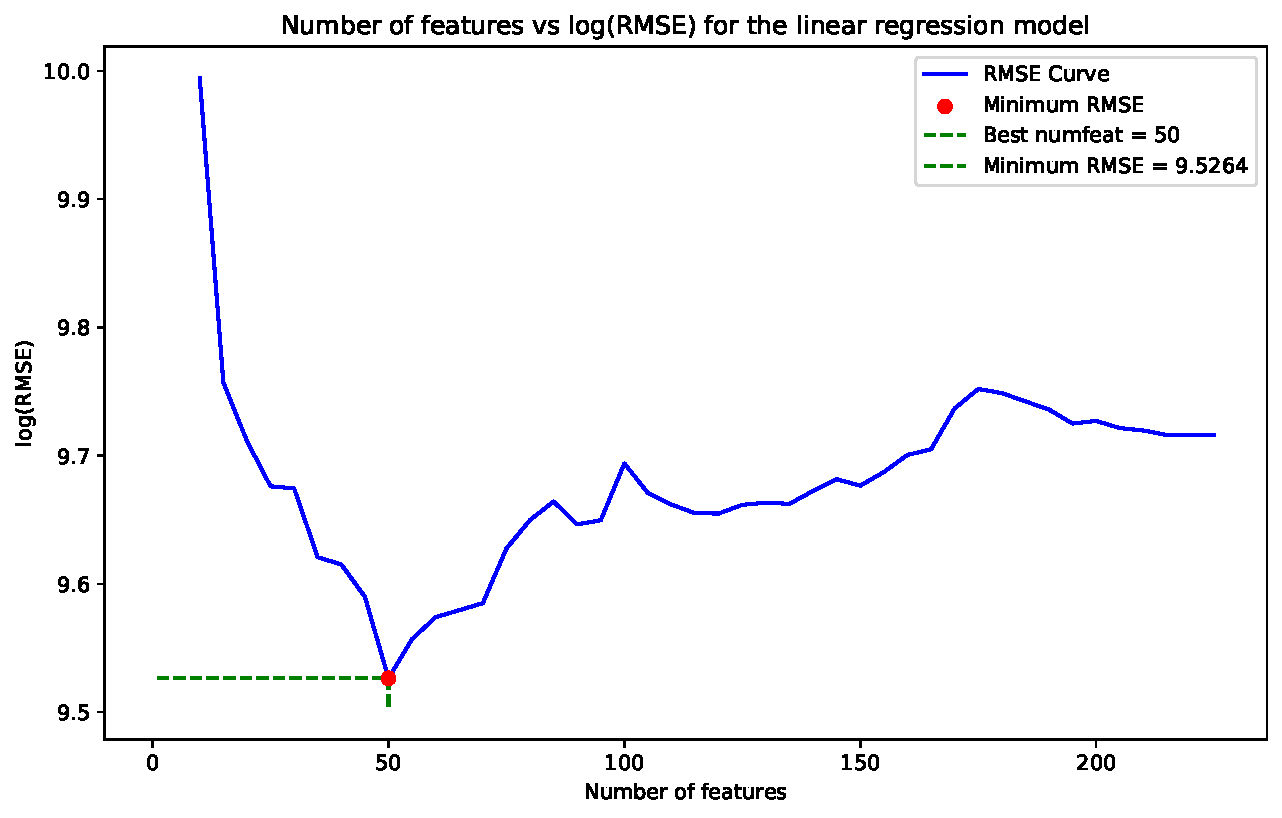
\includegraphics[width = 0.40\textwidth]{img/rmse_curve_linear_2.pdf}
    \caption{number of features vs log(RMSE) for the Ridge regression}
    \label{num vs rmse}
    
\end{figure}


\item \textit{MLP parameters}: Before finding the best parameters using a grid search, we found the best features for fitting the regression. For the \textit{MLP regressor} we used a \textit{scikit-learn} class called \textit{SelectKbest}\cite{SelectKbest}, to execute this task. We trained and tested the \textit{MLP regressor} increasing the feasible number of features each time, obtaining that the the best number of feature for fitting the regression is 40, as shown in Figure \ref{num vs rmse MLP}. The feature selection has been performed using, as initial guess for the MLP Regressor, the following parameters: \textit{hidden\_layer\_sizes} = (50,), \textit{activation} = \textit{relu}, \textit{alpha} = 0.01 and \textit{max\_iter} = 2000.

\begin{figure}
    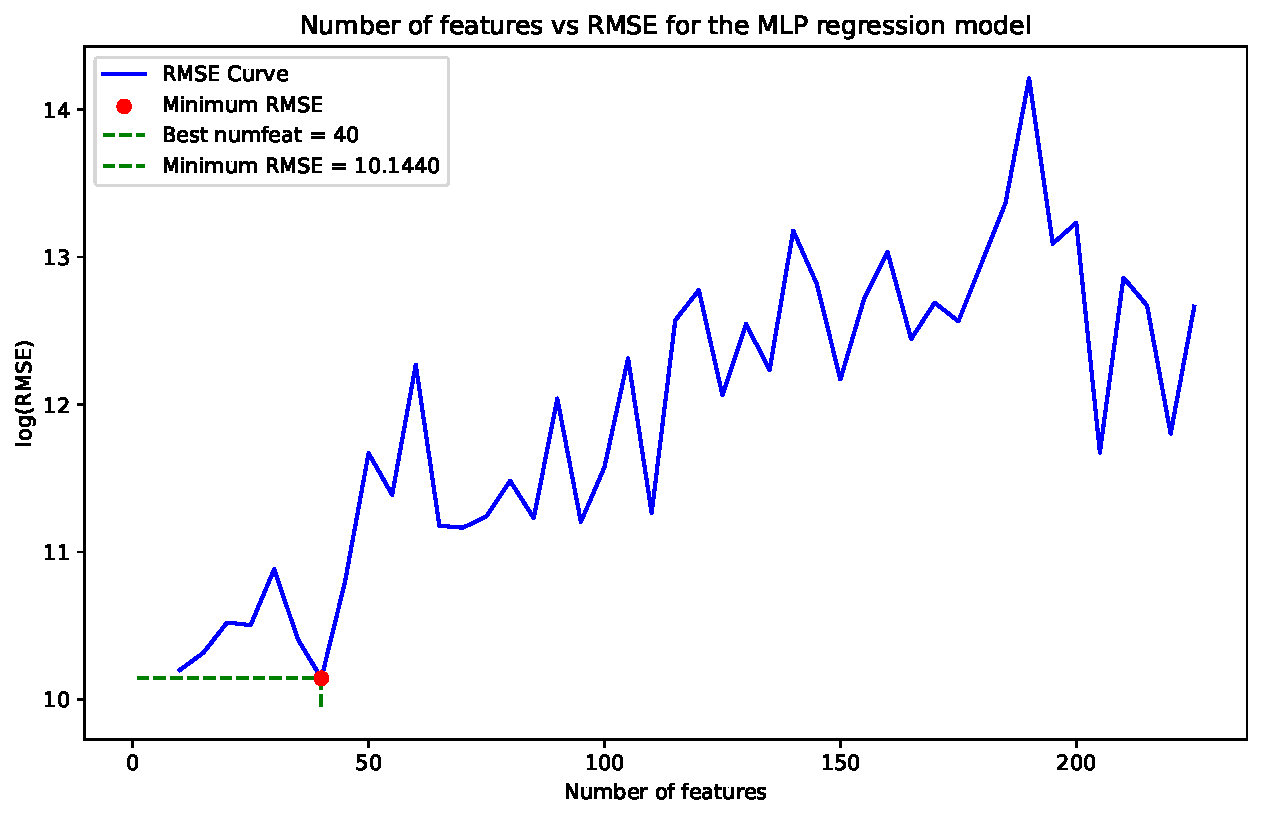
\includegraphics[width = 0.40\textwidth]{img/rmse_mlp_new.pdf}
    \caption{number of features vs log(RMSE) for the MLP regression}
    \label{num vs rmse MLP}
    
\end{figure}

\end{itemize}

After finding the best features for the two models, we applied a grid search for finding the best hyper-parameters, those are shown in the table \ref{tab:hyperparameters}. 

We incorporated the grid search with a 5-fold cross-validation, to ensure greater model robustness. The parameters have been selected by choosing the ones which minimized the mean squared error.

\begin{table}[ht]
    \centering
    \caption{Hyperparameters considered for the grid-search ($n_{tot}$ is the total number of features)}
    \begin{tabular}{@{}lll@{}}
        \toprule
        \textbf{Model} & \textbf{Parameter} & \textbf{Values} \\ \midrule
        Feature Selection & $n_{RI},  n_{MLP}$ & $10
        \to n_{tot}$, step $5$ \\ \midrule
        \multirow{3}{*}{Ridge Regressor} 
            & alpha & \{0.5, 1, 2\} \\
            & fit\_intercept & \{True, False\} \\
            & max\_iter & \{None, 500, 1000\} \\ \midrule
        \multirow{2}{*}{MLP Regressor} 
            & hidden\_layer\_sizes & \{(100,), (100,2), (50,)\} \\
            & activation & \{tanh, logistic, relu\}\\
            & solver & \{adam, lbfgs, sgd\} \\
            & alpha & \{0.001, 0.01, 1\} \\
            & max\_iter & \{1000, 2000\} \\ \bottomrule
    \end{tabular}
    \label{tab:hyperparameters}
\end{table}

